%----------------------------------------------------------------------------------------
%    PACKAGES AND THEMES
%----------------------------------------------------------------------------------------

\documentclass[aspectratio=169,xcolor=dvipsnames]{beamer}
\usetheme{SimpleDarkBlue}

\usepackage[utf8]{inputenc}
\usepackage[czech,english]{babel}
\usepackage{hyperref}
\usepackage{graphicx} % Allows including images
\usepackage{booktabs} % Allows the use of \toprule, \midrule and
% \bottomrule in tables

%----------------------------------------------------------------------------------------
%    TITLE PAGE
%----------------------------------------------------------------------------------------

\title{Semestrální práce z UMM}

\author{Pavel Altmann, Šimon Duda, Jakub Vokoun}

\institute
{
  Fakulta aplikovaných věd \\
  Západočeská univerzita v Plzni
}
\date{\today} % Date, can be changed to a custom date
\def\CC{{C\nolinebreak[4]\hspace{-.05em}\raisebox{.4ex}{\tiny\bf ++}}}

%----------------------------------------------------------------------------------------
%    PRESENTATION SLIDES
%----------------------------------------------------------------------------------------

\begin{document}

\begin{frame}
  \titlepage
\end{frame}

\begin{frame}{Overview}
  \tableofcontents
\end{frame}

%------------------------------------------------
\section{Úvod}
%------------------------------------------------
\begin{frame}{Zadání a co jsme chtěli}
  \begin{itemize}
    \item Vyzkoušet si základní mechanické simulace
    \item Naučit se dělat \uv{fyziku} do her
    \item Potřeba real-time výpočtů
    \item Cíl: Simulace odpružení jednoduchého vozidlo
  \end{itemize}
\end{frame}
%------------------------------------------------
\begin{frame}{Urychlení a zjednodušení}
  \begin{columns}[c]
    \column{.45\textwidth}
    \begin{itemize}
      \item Odloučení grafického modelu a mechanické simulace
      \item Zjednodušení modelu mechanické simulace
      \item Předpočítaná řešení
      \item Nahrazení složitých jevů konstantou, např. odpor vzduchu a tření
    \end{itemize}

    \column{.45\textwidth}
    \begin{figure}
      \centering
      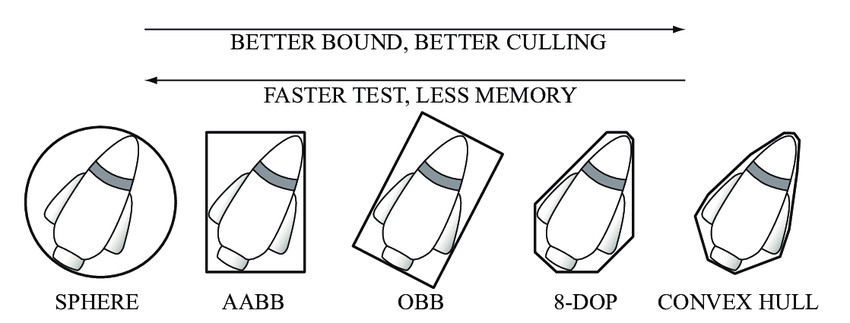
\includegraphics[width=1\linewidth]{img/BoundingBoxes.png}
      \caption{Typy kolizních tvarů}
    \end{figure}
  \end{columns}
\end{frame}
%------------------------------------------------
\section{Slepé cesty}
%------------------------------------------------
\begin{frame}{Unity}
  \begin{columns}[c]
    \column{.45\textwidth}
    \begin{itemize}
      \item Herní engine Unity
      \item Nabízí většinu \uv{fyziky} již vyřešenou
      \item \uv{Bylo by to moc snadné}
    \end{itemize}

    \column{.45\textwidth}
    \begin{figure}
      \centering
      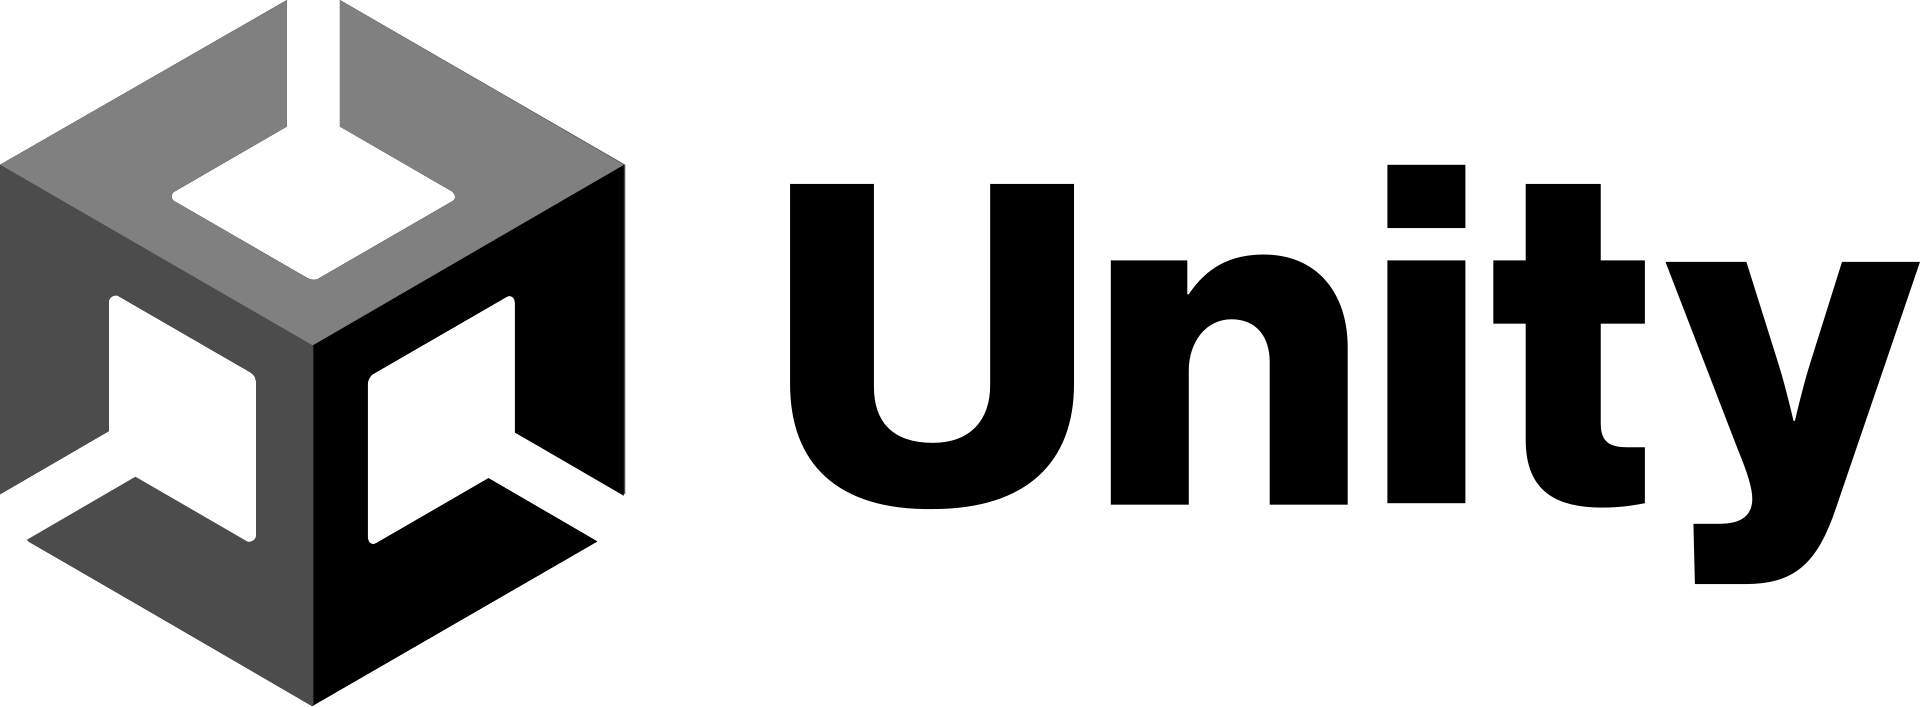
\includegraphics[width=1\linewidth]{img/unity.png}
    \end{figure}
  \end{columns}
\end{frame}
%------------------------------------------------
\begin{frame}{Raylib}
  \begin{columns}[c]
    \column{.45\textwidth}
    \begin{itemize}
      \item Knihovna napsaná v C
      \item Binding do různých jazyků, v našem případě \CC
      \item Postavena nad OpenGL
      \item Nemá vlastní \uv{fyziku}
    \end{itemize}

    \column{.45\textwidth}
    \begin{figure}
      \centering
      
\includegraphics[width=1\linewidth]{img/Raylib.png}
    \end{figure}
  \end{columns}
\end{frame}
%------------------------------------------------
\begin{frame}{Auto}
  \begin{figure}
    \centering
    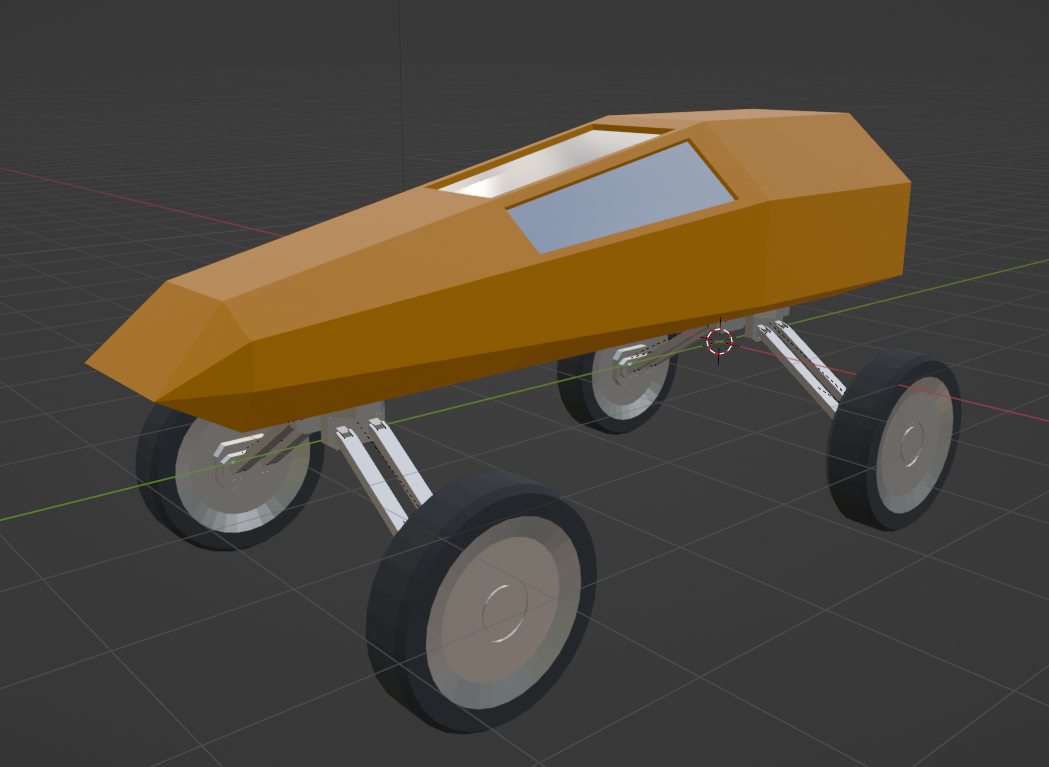
\includegraphics[width=0.6\linewidth]{img/auto.png}
    \caption{\uv{Auto}}
  \end{figure}
\end{frame}
%------------------------------------------------
\begin{frame}{Motocykl}
  \begin{figure}
    \centering
    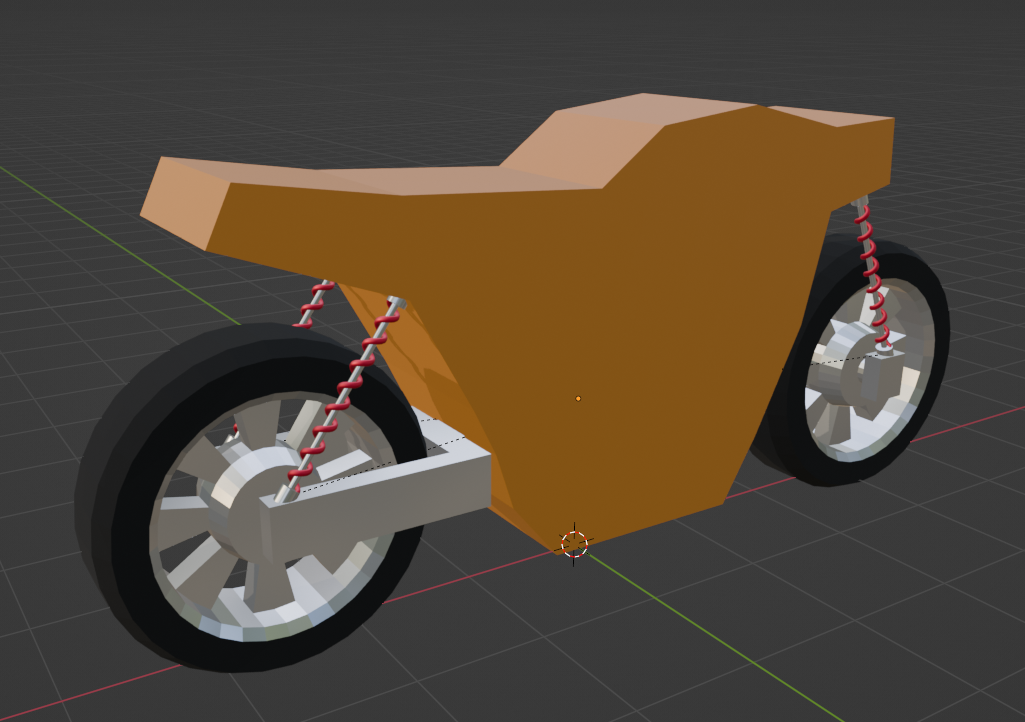
\includegraphics[width=0.6\linewidth]{img/motorcycle.png}
    \caption{\uv{Motocykl}}
  \end{figure}
\end{frame}
%------------------------------------------------

%------------------------------------------------
\section{Simulace}
%------------------------------------------------
\subsection{Diferenciální rovnice a numerické metody}
\begin{frame}{Diferenciální rovnice}
  \begin{itemize}
    \item Diferenciální rovnice popisují změnu
    \item Jednoduché se dají řešit analyticky
    \item Složitější (náš případ) lze řešit pouze numericky
  \end{itemize}
  \vspace{0.25cm}
  \cite{hirsch1970}
\end{frame}
%------------------------------------------------
\begin{frame}{Numerické metody řešení diferenciálních rovnic}
  \begin{itemize}
    \item Obecně využívají lokální aproximace jednodušší funkcí
    \item Jejich přesnost je závislá mj. na velikost kroku
    \item Nejjednodušší je Eulerova metoda -- aproximuje lineární funkcí podle
      derivace
    \item Stačí na jednoduché simulace jako platformery, apod.
    \item Jiné metody používají více kroků a složitější aproximační funkce
    \item Více viz předmět KMA/NM \cite{prikryl_brandner}
  \end{itemize}
\end{frame}
%------------------------------------------------
\subsection{Čas}
\begin{frame}{Čas}
  \begin{itemize}
    \item Simulaci i grafiku je nutné vyhodnocovat v diskrétních časových bodech
    \item Pro jednoduché případy mohou být stejné
      (\uv{posunu objekty a vykreslím})
    \item Pro lepší výsledky by měly být nezávislé
      \begin{itemize}
        \item grafika co nejčastěji podle výkonu
        \item simulace co nejpravidelněji v čase
      \end{itemize}
      \vspace{0.25cm}
      \cite{eberly2010}
  \end{itemize}
\end{frame}
%------------------------------------------------
\section{Mechanika}
%------------------------------------------------
\subsection{Tuhé těleso}
\begin{frame}{Tuhé těleso}
  \begin{itemize}
    \item Idealizované těleso, které působením sil nemění svůj tvar ani objem
    \item My předpokládáme i složení z homogenního a izotropního materiálu
    \item Používá se obecně pro zjednodušení modelování
      \vspace{0.5cm}
    \item K popisu je potřeba 6 parametrů:
      \begin{itemize}
        \item Hmotnost (konstanta) -- $m$
        \item Poloha -- $\mathbf{x}$
        \item Rychlost nebo hybnost -- $\mathbf{v}$ nebo $\mathbf{P}$
          \vspace{0.25cm}
        \item Tenzor setrvačnosti (konstanta) -- $\mathbf{I}_0$
        \item Natočení -- $\mathbf{R}$
        \item Úhlová rychlost nebo hybnost -- $\mathbf{\omega}$ nebo
          $\mathbf{L}$
      \end{itemize}
      \vspace{0.25cm}
      \cite{witkin1997}
      \cite{hecker1997}
      \cite{blackedout01_rigid_body}
  \end{itemize}
\end{frame}
%------------------------------------------------
\begin{frame}{Tuhé těleso}
  \begin{itemize}
    \item V každém kroku vypočítáme jejich změnu:
      \begin{itemize}
        \item Hybnost -- $\mathbf{dP} = \mathbf{F}_{net} \cdot dt$
        \item Poloha -- $\mathbf{dx} = \mathbf{v} \cdot dt$, kde $\mathbf{v} =
          \frac{\mathbf{P}}{m}$
          \vspace{0.5cm}
        \item Úhlová hybnost -- $\mathbf{dL} = \mathbf{\tau}_{net} \cdot dt$
        \item Natočení -- $\mathbf{dR} = \mathbf{\omega}^* \mathbf{R}$, kde
          $\mathbf{\omega} = \mathbf{I}^{-1} \mathbf{L}$, kde $\mathbf{I} =
          \mathbf{R} \mathbf{I}_0 \mathbf{R}^T$
      \end{itemize}
      \vspace{0.5cm}
      \begin{equation}
        \mathbf{a}^* \mathbf{R} =
        \begin{bmatrix}
          \mathbf{a} \times
          \begin{bmatrix} r_{xx} \\ r_{xy} \\ r_{xz}
          \end{bmatrix} &&
          \mathbf{a} \times
          \begin{bmatrix} r_{yx} \\ r_{yy} \\ r_{yz}
          \end{bmatrix} &&
          \mathbf{a} \times
          \begin{bmatrix} r_{zx} \\ r_{zy} \\ r_{zz}
          \end{bmatrix}
        \end{bmatrix}
      \end{equation}
      \vspace{0.25cm}
      \cite{witkin1997}
      \cite{blackedout01_rigid_body}
  \end{itemize}
\end{frame}
%------------------------------------------------
\subsection{Pružiny}
\begin{frame}{Pružiny}
  \begin{itemize}
    \item Předpokládáme Hookův zákon
  \end{itemize}
  \begin{equation}
    \mathbf{F} = -k\,\mathbf{r} - \mu\,\mathbf{v}
  \end{equation}
  \vspace{0.25cm}
  \cite{kopcil_trejbalova}
  \cite{kiesslich_2d_physics}
\end{frame}
%------------------------------------------------
\subsection{Polyhedron}
\begin{frame}{Vlastnosti polyhedronu}
  \begin{itemize}
    \item Uvažujeme homogenní polyhedron definovaný trojúhelníkovou sítí = 3D
      model
    \item Lze pro něj z hustoty $\rho$ vypočítat:
      \begin{itemize}
        \item hmostnost $m$,
        \item těžiště $\mathbf{C}_t$ a
        \item tenzor setrvačnosti $\mathbf{I}$ -- popisuje setrvačnost tělesa
          při obecném pohybu
      \end{itemize}
      \vspace{0.25cm}
      \cite{mirtich1997}
      \cite{tonon2004}
  \end{itemize}
\end{frame}
%------------------------------------------------
\begin{frame}{Objem polyhedronu}
  \begin{figure}
    \centering
    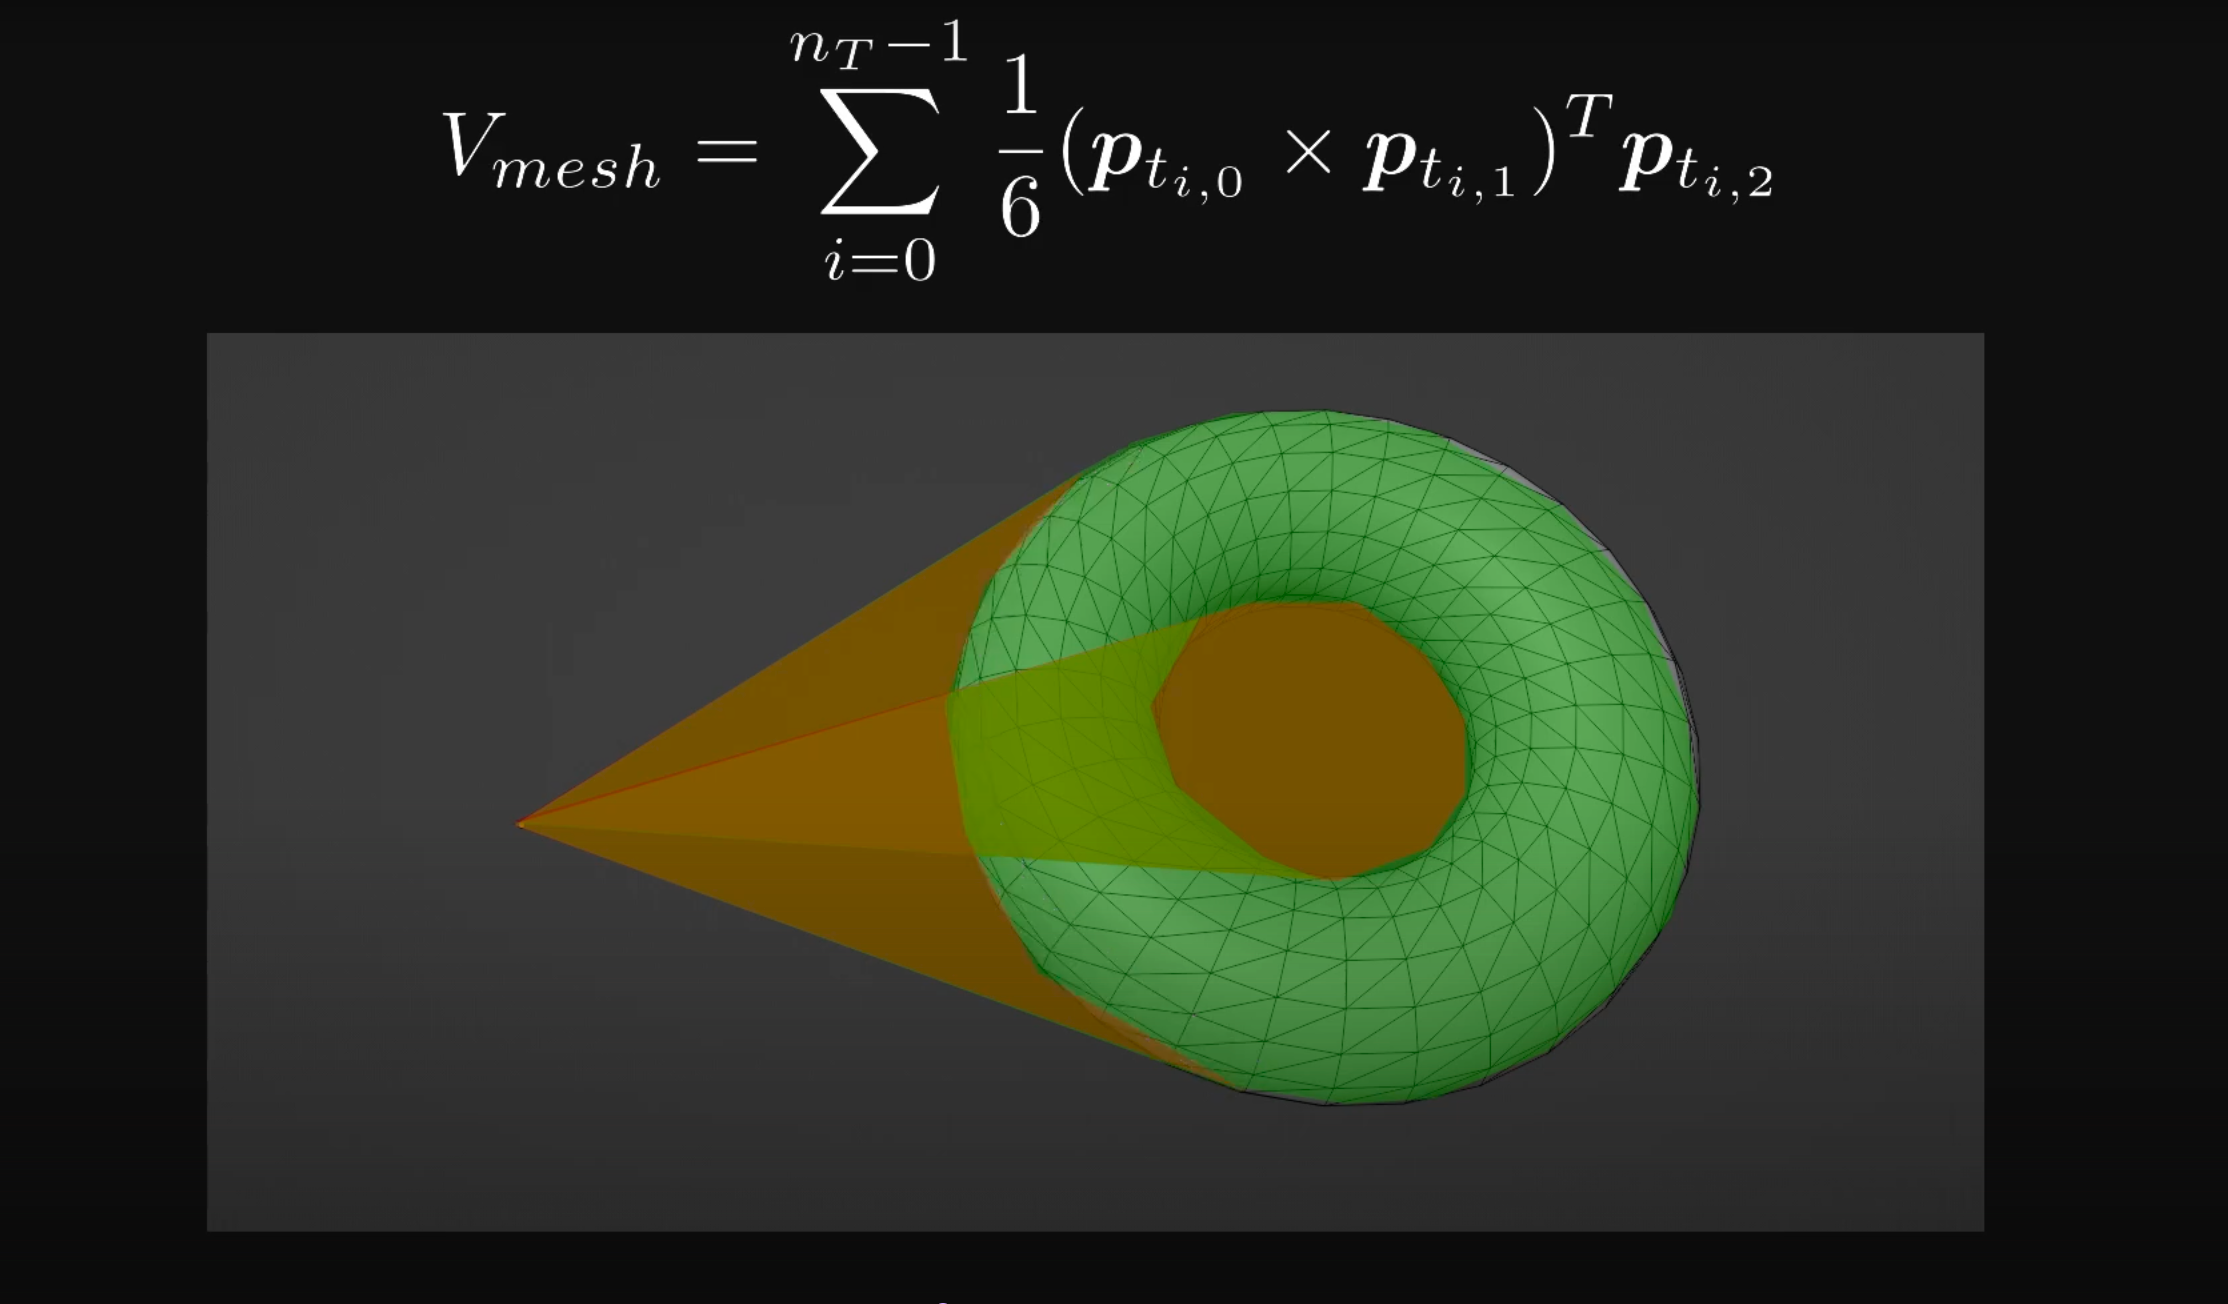
\includegraphics[width=0.8\linewidth]{img/donut_volume.png}
    \caption{Objem polyhedronu \cite{blackedout01_inertia_tensor}}
  \end{figure}
\end{frame}
%------------------------------------------------
\begin{frame}{Výpočet}
  \begin{enumerate}
    \item Pro každý trojúhelník sítě zkonstruujeme čtyřstěn
      \begin{itemize}
        \item Čtvrtý bod může být libovolný, nakonec se vykrátí
        \item Spočítáme jeho hmotnost, těžiště a tenzor setrvačnosti
      \end{itemize}
    \item Těžiště celého polyhedronu je průměr těžišť jednotlivých trojúhelníků
    \item Pomocí Steinerovy věty přesuneme osy otáčení čtyřstěnů do těžiště
      tělesa
    \item Takto upravené setrvačnosti sečteme
  \end{enumerate}
  \vspace{0.25cm}
  \cite{blackedout01_inertia_tensor}
  \cite{tonon2004}
\end{frame}
%------------------------------------------------
\subsection{Kolize}
\begin{frame}{Kolizní tvar}
  \begin{itemize}
    \item Kvádr
    \item Koule
    \item Trojúhelníková síť
  \end{itemize}
  \vspace{0.25cm}
  \cite{press2007}
\end{frame}
%------------------------------------------------
\begin{frame}{Vyhodnocení kolize}
  \begin{enumerate}
    \item Vypočítá se velikost impulzu $j$
      \begin{equation}
        j = \frac{-(1 + \epsilon) \mathbf{v}_r \cdot \mathbf{n}}{m_1^{-1} +
          m_2^{-1} + \mathbf{n} \cdot \left(
            \left( \mathbf{I}_1^{-1} (\mathbf{r}_1 \times \mathbf{n})
            \right) \times
            \mathbf{r}_1 + \left( \mathbf{I}_2^{-1} (\mathbf{r}_2
            \times \mathbf{n}) \right) \times
            \mathbf{r}_2
        \right)}
      \end{equation}
    \item Vypočítá se vektor směru impulzu $\mathbf{j} = j \cdot \mathbf{n}$
    \item Vypočítá se nová rychlost tělese $\mathbf{v'} = \mathbf{v}
      \pm \frac{1}{m} \cdot \mathbf{j}$
    \item Vypočítá se nová úhlová rychlost tělesa
      $\mathbf{\omega'} = \mathbf{\omega} \pm j \cdot
      \mathbf{I}^{-1}(\mathbf{r} \times \mathbf{n})$
  \end{enumerate}
  \vspace{0.25cm}
  \cite{wikipedia_collision_response}
  \cite{leitner2019}
\end{frame}
%------------------------------------------------
\section{Závěr}
%------------------------------------------------
\begin{frame}[allowframebreaks] {Zdroje}
  \footnotesize
  \bibliography{reference.bib}
  \bibliographystyle{alpha}
\end{frame}
%------------------------------------------------

\end{document}
